% Don't report over-full \bv-boxes if over-edge is small
% topmargin is 1/2 inch (note negative value)
% left margin is 1 inch on right-hand pages
% same for left-hand pages in \AtBeginDocument
% leaves 1 inch for the right margin
% 9 inches reserved for the text.
% THEOREM Environments ---------------------------------------------------
% MATH -------------------------------------------------------------------
%\DeclareMathOperator{\RE}{Re}
%\DeclareMathOperator{\IM}{Im}
%\DeclareMathOperator{\ess}{ess}
%\newcommand{\X}{\mathcal{\bfX}}
%% Maxims' commands
%\newcommand{\bu} {\mathbf{u}}
%\newcommand{\bv} {\mathbf{v}}
%\def\cdt{{\hskip-0.08ex\cdot\hskip-0.08ex}}
%%% ----------------------------------------------------------------------

\documentclass[12pt]{article}%
\usepackage{amsmath, amssymb, amsbsy, amsthm}
\usepackage{epsfig}
\usepackage{wrapfig}
\usepackage{color,cancel}
\usepackage{fullpage}
\usepackage{float}
\usepackage{ulem}
\usepackage{setspace}
\usepackage{caption}
\usepackage{subcaption}
\usepackage{hyperref}

\DeclareMathOperator{\diam}{diam}
\newcommand{\vecb}[1]{\mathbf{#1}}

\vfuzz2pt
%\topmargin=-.5in
%\oddsidemargin=0.5in
%\evensidemargin=0.5in
%\textwidth=6.in
%\textheight=9.1in

\date{}

\title{Image Segmentation}


\author{
 Nathan D. Heavner
      \and
  Rachel Tutmaher
  	\and
	James Folberth
}

\begin{document}


\maketitle

% TODO we should cite Inglis et al. somewhere early on in the report.
\section{Introduction}
There are large amounts of data and images that are being generated today; sources include satellite imagery, medical imaging such as MRIs or CT scans, and social media. An automated process that can scan an image for significant objects or figures is greatly desired and is therefore a topic of much current research. Image segmentation algorithms involve reading in an image, converting the image to a matrix of pixel values, and grouping similar pixels together with the goal of identifying objects in single images and tracking the objects in the sequences of images.  This will ideally allow for a greater number of images to be processed more quickly than is currently possible. However, this is a complicated task.  It is difficult to design an algorithm that correctly identifies shapes and groups them accordingly.  It is obviously undesirable to segment an object that should not be segmented, or on the other hand, to not ``aggregate" an entire object properly. 
\vspace{5mm} \\
The algorithm that we investigated for our project was specifically developed to track live cells imaged with bright field cell microscopy.  Both the movement of the cell through space and its evolution through time (cell growth and division) were qualities that needed to be captured with an image segmentation routine.  Other examples of image segmentation involve satellite imagery where roads, buildings, or even people may need to be identified.  The sheer quantity of images and pictures that need to be analyzed and categorized for various reasons makes finding an accurate and fast automated image segmentation algorithm a necessity.
\vspace{5mm} \\
Typically, once the image to be analyzed has been converted to a matrix of pixel values, these pixel values are used to determine the ``intensity" of each pixel.  Then, neighboring pixels are grouped together based upon whether they have similar intensities.  This process continues until ``aggregates" are formed.  An aggregate is a lump of neighboring pixel values that have been segmented together, the hope being that this aggregate represents an object in the original image. This process assumes objects in an image will have similar grayscale pixel values, which is most often the case. The size of the matrix with dimension being the number of vertical pixels by the number of horizontal pixels affects the speed and cost of the algorithm.  There is a large class of algorithms that are being designed to process images and segment them.  The method that we employ involves techniques from (Ruge-St\"uben) Algebraic Multigrid methods (AMG); specifically it involves altering the ``Segmentation by Weighted Algorithm" (SWA) technique.  This new method is favorable because initial testing by Inglis et al. claims that the algorithm's runtime is \emph{linear} in the number of pixels!\\

We implemented this algorithm in C++, Julia, and Matlab and compared results.  The results shown in this report are from the Julia and C++ code implementations.  The main difference in the algorithm that is used in this project from other similar algorithms is that there is a ``scale-invariant saliency measure." This measure decides when an aggregate represents an entire object and should not be further grouped with other pixels  surrounding it.  The prominence of an aggregate is the main identifier of individual objects within an image.

\section{Algorithm Description and Implementation}
Although, the algorithm used here is based on AMG and SWA, the final segmentation for this algorithm is determined by one image segmentation V-cycle, which is different from regular SWA where many V-cycles may be used.  Also, a measure of ``texture", obtained by varying the mean intensities at each level improves performance of cell segmentation, the main goal of the algorithm that we chose to implement. We also tested the algorithm on other objects. Significant fine-tuning in the segmentation results is made possible by the relatively large number of parameters that this algorithm calls for. The overall goal of this algorithm is to assign every pixel in the original image to an aggregate, therefore adequately segmenting a given image hopefully into segments that may be subsequently analyzed. In order to achieve this goal, the algorithm flows as follows.
\vspace{5mm}\\
First the finest level variables are defined. Among these are an intensity vector. This vector contains all of the intensity values from the original image (either column-wise or row-wise ordering) and the vector is rescaled so that the intensities range from $0$ to $1$.  Additionally, a coupling matrix is created in the following manner: 

$$ A_{ij} = \begin{cases} e^{-\alpha(I_i-I_j)} &\mbox{if } i, j \mbox{\ \ are neighbors} \\ 0 & \mbox{else. } \end{cases} $$ 

\noindent This transforms the problem of segmenting an image into the problem of segmenting a graph, where the nodes are the intensities of each pixel and the edge weights are given by the coupling matrix.
\vspace{5mm} \\
Next the graph is coarsened repeatedly until everything has been segmented. Blocks are checked for saliency at each level.  A salient block is one which is ``significantly" different from its surroundings within the matrix, meaning that the connections within the block are much stronger than the connections from any other neighbors. Once it has been determined that a block is ``salient" it will not merge with any other blocks on coarser levels, however these blocks are propagated through all the levels in the down side of the V-cycle.  The edge weights which play a part in determining saliency with neighboring nodes are calculated via Galerkin coarsening.  % James isn't sure that's what we call it, but he could be wrong
\vspace{5mm} \\
Once the coarsest level is reached, the upward part of the V-cycle begins, the goal being to uniquely assign every finest-level pixel to one of the segments.  Segments that are acquired on the coarsest level relate to overlapping blocks on the top level.  Since a pixel may originally be classified as belonging to a certain block at the finest level and then later be reclassified at the coarsest level, it is vital that the salient blocks are retained throughout the coarse level progression so that that original relationship is maintained throughout the V-cycle. Once all segments have been found, nodes on the next finer level are assigned to segments on the coarser level according to weights in the interpolation matrix. This is repeated up to the original finest level. On each level, the overlap between segments is refined by the following threshold determining by a sharpening threshold.  Nodes that belong for more than 85\% to a segment are assigned 100\% to that segment, while nodes that belong for less than 15\% to a segment are fully decoupled from that segment. Once the algorithm reaches the finest level of the V-cycle, a post-processing step uniquely assigns each pixel to a segment.


% TODO we now have two different implementations.  We must be very clear which method we used to produce each segmentation.
\section{Results}

Our code is available online at \url{https://github.com/jamesfolberth/multigrid_project}.\\

In this section, we demonstrate the efficacy of the segmentation algorithm. We first demonstrate in Figure~\ref{fig:disk} the improvement in segmentation accuracy obtained by taking multilevel intensity variance into account. The image in Figure~\ref{fig:disk} contains two segments which have different textures (variance within the segment) but identical average intensities. When we do not take multilevel variance into account, the algorithm detects only one segment. When we rescale the weighting matrix using the variance of each block, however, the two segments are successfully detected.\\

% Nathan used the max-element strong connection method for these images.
Regarding the checkered disk image, it should be noted that \cite{inglis:2010} states that the off-diagonal row sum is used to determine the strong connections when coarsening the graph.  We were unable to recreate their results using their parameters with the off-diagonal row sum method, but if we instead used the more standard max-element method to determine the strong connections, their parameters and our implementation produced the desired results.\\

\begin{figure}[ht]
\centering

\includegraphics[width=0.2\textwidth,height=0.2\textwidth]{checker_disk_good_seg_1.png} \hspace{.45cm}

\includegraphics[width=0.2\textwidth,height=0.2\textwidth]{checker_disk_good_seg_2.png}
\caption{Without taking multilevel variance into account, the algorithm detected only one segment (the entire image). Rescaling the weighted graph using multilevel variance results in the segmentation shown above. Parameters used: $n = 60$, $\alpha = 10$, $\tilde{\alpha} = 10$, $\beta = 10$, $\theta = 0.1$, $\gamma = 0.1$, $d_1 = 0.15$, $\sigma = 5$, $\rho = 1$, and the coarsening presented in \cite{inglis:2010}.  Implementation: C++.}
\label{fig:disk}
\end{figure}

Next, we demonstrate the effect of making the saliency measure invariant of the segment scale by normalizing the similarity-weighted boundary length and area. With the usual saliency measure, it is much harder for the algorithm to detect the segments because the boundary length is much greater than the segment area compared to a simpler shape such as a circle. With the author's proposed scale invariant measure, the segment is easily detected.\\

\begin{figure}[ht]

\begin{subfigure}[b]{\textwidth}
\centering

\includegraphics[width=0.2\textwidth,height=0.2\textwidth]{spiral_bad_seg_1.png} \hspace{.45cm}

\includegraphics[width=0.2\textwidth,height=0.2\textwidth]{spiral_bad_seg_2.png} \hspace{.45cm}

\includegraphics[width=0.2\textwidth,height=0.2\textwidth]{spiral_bad_seg_3.png}
\subcaption{Segmentation without scale invariant saliency measure.}
\end{subfigure}

\vspace{.45cm}

\begin{subfigure}[b]{\textwidth}
\centering

\includegraphics[width=0.2\textwidth,height=0.2\textwidth]{spiral_good_seg_1.png} \hspace{.45cm}

\includegraphics[width=0.2\textwidth,height=0.2\textwidth]{spiral_good_seg_2.png}
\subcaption{Segmentation with scale invariant saliency measure.}
\end{subfigure}

\caption{Parameters used: $n = 64$, $\alpha = 10$, $\tilde{\alpha} = 10$, $\beta = 10$, $\theta = 0.09$, $\gamma = 0.08$, $d_1 = 0.15$, $\sigma = 7$, $\rho = 1$, and the coarsening presented in \cite{inglis:2010}.  Implementation: Julia.}
\label{fig:spiral}

\end{figure}

The remaining figures demonstrate the performance of the algorithm with more complex images. The performance is quite good. In the cases where the segmentation is ``incorrect," we can reasonably attribute this to human intelligence rather than algorithm performance. In Figure~\ref{fig:peppers}, for example, one segment includes the fruit from one pepper and the stem from another. From a purely visual perspective, these segments look very reasonable. It's only because humans know that the stem and fruit go together, and must be arranged in a particular orientation, that we would segment the image differently from the algorithm.\\

\begin{figure}[ht]
\centering
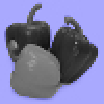
\includegraphics[width=0.2\textwidth,height=0.2\textwidth]{peppers_seg_1.png} \hspace{.45cm}
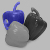
\includegraphics[width=0.2\textwidth,height=0.2\textwidth]{peppers_seg_2.png} \hspace{.45cm}

\includegraphics[width=0.2\textwidth,height=0.2\textwidth]{peppers_seg_3.png} \\ \vspace{.45cm}
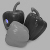
\includegraphics[width=0.2\textwidth,height=0.2\textwidth]{peppers_seg_4.png} \hspace{.45cm}

\includegraphics[width=0.2\textwidth,height=0.2\textwidth]{peppers_seg_5.png}
\caption{Parameters used: $n = 50$, $\alpha = 50$, $\tilde{\alpha} = 4$, $\beta = 10$, $\theta = 0.1$, $\gamma = 0.15$, $d_1 = 0.15$, $\sigma = 5$, $\rho = 1$, and the coarsening presented in \cite{inglis:2010}.  Implementation: Julia.}
\label{fig:peppers}
\end{figure}


\begin{figure}[ht]
   \centering
   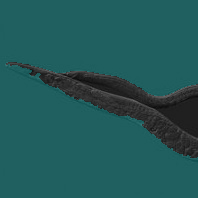
\includegraphics[width=0.2\textwidth]{two_c_elegans_seg_blend_0000.png} \hspace{0.45cm}
   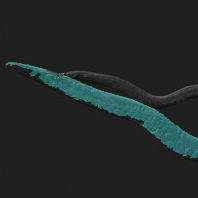
\includegraphics[width=0.2\textwidth]{two_c_elegans_seg_blend_0001.png} \hspace{0.45cm}
   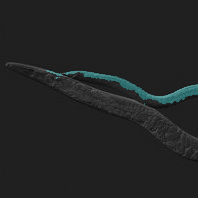
\includegraphics[width=0.2\textwidth]{two_c_elegans_seg_blend_0002.png} \hspace{0.45cm}
   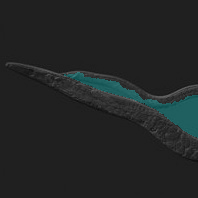
\includegraphics[width=0.2\textwidth]{two_c_elegans_seg_blend_0003.png}
   % 2., 25., 2., 0.05, 0.05, 0.10, 7, 1)
   \caption{This is a microscope image of anterior portion of two C. Elegans.  Parameters used: $n = 198$, $\alpha = 2$, $\tilde{\alpha} = 25$, $\beta = 2$, $\theta = 0.05$, $\gamma = 0.05$, $d_1 = 0.1$, $\sigma = 7$, $\rho = 1$, and the standard RS AMG coarsener.  Implementation: C++.}
   \label{fig:c_elegans}
\end{figure}


One weakness of the algorithm, mentioned by the authors, is the large number of parameters and difficulty in choosing them correctly. Currently, parameters are chosen by guessing and checking, which obviously presents a large obstacle to the algorithm's robustness and usefulness in industrial applications. There are, however, some general guidelines that can be used to improve the segmentation accuracy.\\

\begin{enumerate}

\item If the image has low contrast levels, increase the first-level intensity scaling factor $\alpha$. This amplifies the difference in intensity between two nodes in the weighted graph matrix.

\item If the image segments are likely to be bordered by very dark or bright regions (as is the case with bright field microscopy cell images), there is a chance that these borders will become salient segments themselves. To avoid this, decrease the coarse-level rescaling factor $\tilde{\alpha}$, since a large $\tilde{\alpha}$ causes nodes with high average intensity to become more disconnected from their neighbors.

\item If the algorithm detects too many segments, then several parameter changes may be beneficial. Decreasing $\theta$ yields stronger connections between nodes; decreasing $\gamma$ provides a stricter salience threshold; and increasing $\sigma$ prevents segment detection on fine levels. All these changes make it more difficult for nodes to be salient and result in fewer segments.

\end{enumerate}

There are further differences between our implementation of Inglis et al.'s algorithm and their reported results.  We have already mentioned that we were unable to reproduce their results for the checkered disk image with their parameters.  We initially thought that they had simply used the maximal off-diagonal element to determine strong connections, where as they report using the off-diagonal row sum.  However, when performing algorithm runtime scaling experiments, our C++ implementation scaled \emph{quadratically} with the total number of pixels, wheras Inglis et al. report that their implementation scales \emph{linearly} with the number of pixels.  By profiling the C++ implementation, we found that the AMG-like graph coarsening was the bottleneck; indeed, it seems that, as written, the graph coarsening presented in \cite{inglis:2010} scales quadratically with the number of pixels (specifically, step 6, part a of the coarsening function).  By pre-sorting the vector of node weights $\lambda$, we might be able to reduce this cost to something like $\mathcal{O}(n\log n)$, but we have not designed or verified this modification; regardless, this is still sub-optimal scaling compared to the linear scaling presented in \cite{inglis:2010}.\\

We ``hacked'' PyAMG's implementation \cite{pyamg:2011} of standard Ruge-St\"uben AMG into our code.  This, of course, scales linearly with problem size.  Coincidently, using RS AMG instead of Inglis et al.'s coarsening resulted in obtaining the proper segmentation of the checkered disk image using the same parameters.  Since we were unable to reproduce the desired results with our implementation of Inglis et al.'s coarsener, but were able to reproduce the results with the ``wrong'' coarsener (RS AMG), we speculate that there are further errors in our implementations, or perhaps that there is a typographical error in the coarsening algorithm presented in \cite{inglis:2010}.\\  % is this too bold a claim?

We performed a simple runtime scaling experiment to determine how our implementation scaled with problem size.  For this experiment, we use the Ruge-St\"uben AMG coarsener, not the coarsener presented in \cite{inglis:2010}.  In Figure \ref{fig:runtime_scaling} we have plotted the runtime of our C++ implementation versus the total number of pixels for the spiral image.  It is clear that the implementation scales linearly with problem size.  We start with a 512 by 512 image, resize using OpenCV \cite{opencv:2000}, and measure the runtime of running segmentation on the resized image five times.  These computations were done on an Intel(R) Core(TM) i5-2467M CPU @ 1.60GHz.\\


\begin{figure}[ht]
   \centering
   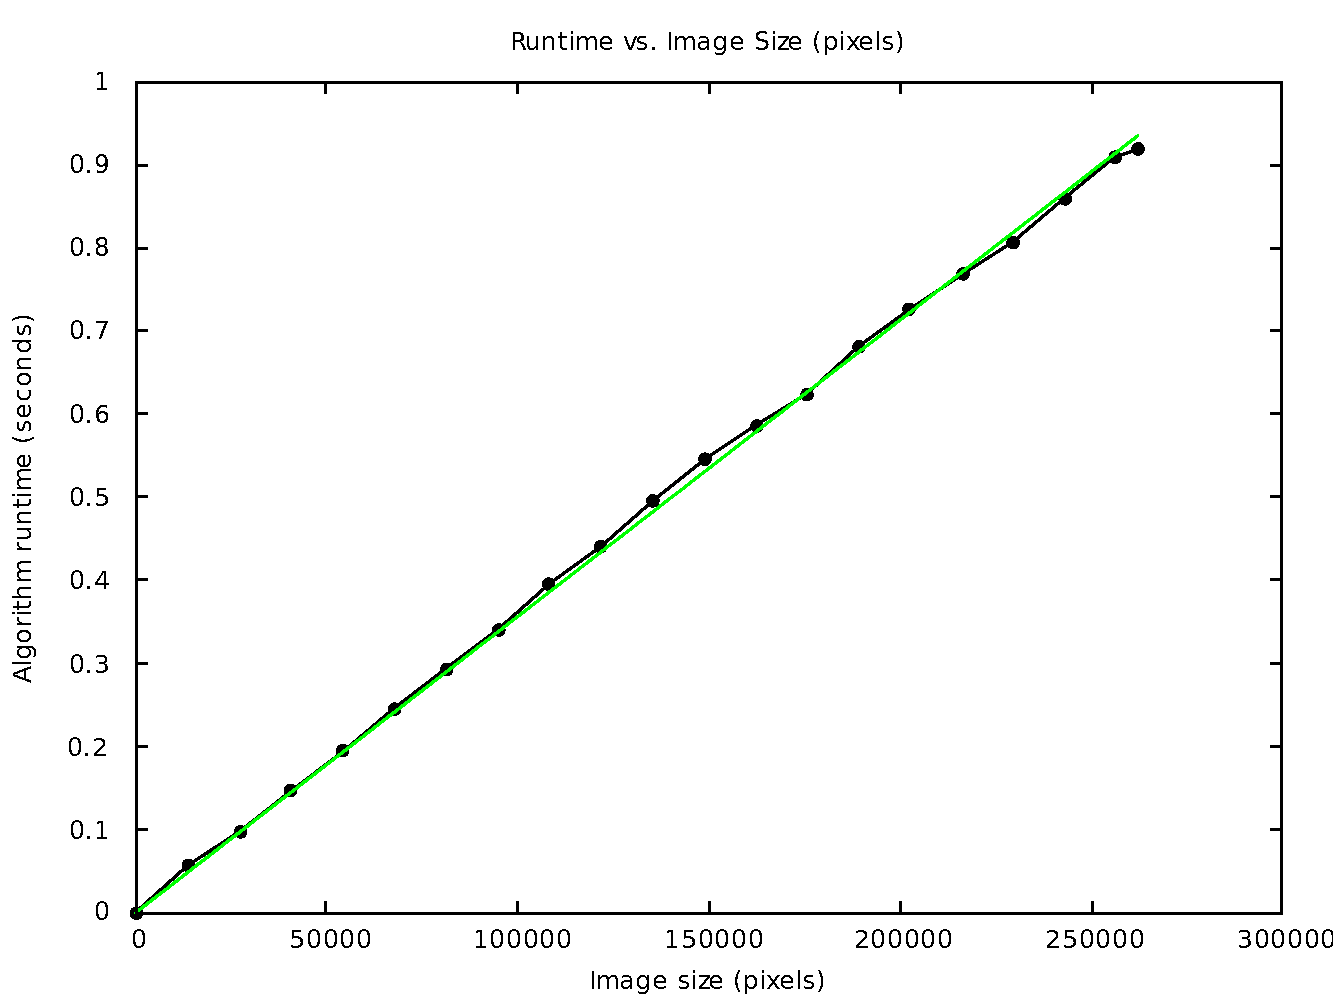
\includegraphics[width=0.7\textwidth]{runtime_scaling_RSAMG_spiral_512_james.pdf}
   \caption{Scaling of the runtime versus the total number of pixels using Ruge-St\"uben coarsening.  Implementation: C++.}
   \label{fig:runtime_scaling}
\end{figure}


\bibliographystyle{siam}
\bibliography{mg_img}

%\section{References}
%\begin{enumerate}
%\item R. Basri, A. Brandt, and E. Sharon, ``Fast Multiscale Image Segmentation," The Weizmann Institute of Science, Rehov ot, Israel, 2000.
%\item G. Sanders, T. Inglis, H. De Sterck, H. Djambazian, R. Sladek, S. Sundararajan, and T. Hudson, ``Mulitlevel Space-Time Aggregation for Bright Field Cell Microscopy Segmentation and Tracking," \textit{International Journal of Biomedical Imaging}, vol. 2010, article ID 582760, 2010.
%\end{enumerate}

\end{document}

%%% Local Variables: 
%%% mode: latex
%%% TeX-master: t
%%% End: 
